\section{\TwoLevelIndex{}}
\label{index}

In this paper, we aim to solve \probdef{} problems with a novel \twolevelindex{}. We describe the structure and construction of the \twolevelindex{} in this section. Then We show how to use the \twolevelindex{} to process various kinds of k-truss community queries in the next section.

%\subsection{Overview}
The index proposed in this paper contains two levels. The top level index provides information at the community level while the bottom level index offers information at the edge level. The top level is a super-graph, called \treeindex{}, whose vertices represent unique k-truss communities and edges represent containment relations between k-truss communities. The bottom level is a maximum spanning forest of a \inducedgraph{} that preserves the edge level trussness and triangle connectivity inside k-truss communities. An overview of the index is shown in \autoref{fig:illustration_main}. 

The index is constructed in a bottom-up manner. In the following, we first formally define the \inducedgraph{} and introduce the algorithm of constructing it from the original graph (Section~\ref{bottom-level}). Then we introduce the \treeindex{} and show how to use simple graph traversals on the \inducedgraph{} to create the \treeindex{} (Section~\ref{top-level}). Finally, we show the structure we used for the \twolevelindex{} to combine the \inducedgraph{} and the \treeindex{} (Section~\ref{structure}).

\subsection{\InducedGraph{}}
\label{bottom-level}
%\usernote{use counting sort}
The \inducedgraph{} of an original graph $G^o$ is obtained by associating a vertex with each edge of $G^o$ and connecting two vertices if the corresponding edges of $G^o$ belong to the same triangle. Then we only store a maximum spanning tree of the \inducedgraph{} to save edge level structures of k-truss communities in the original graph. By using a maximum spanning forest of the \inducedgraph{} as the bottom level index, we can use minimum edge enumerations to replace computational expensive triangle enumerations at query time. We show the formal definition of the \inducedgraph{} in \autoref{def:\inducedgraph{}}.

\begin{Def}[\Inducedgraph{}]
The \inducedgraph{} $G^t$ is a weighted undirected graph that each edge in the original graph $G^o$ is represented as a vertex in $G^t$. $G^t$ has an edge $e^{t}$ connecting vertices $v^{t}_{1}, v^{t}_{2} \in G^{t}$ if and only if their corresponding edges $e^{o}_{1}, e^{o}_{2} \in G^{o}$ belong to the same triangle in $G^o$. The weight of a vertex in $G^{t}$ is the trussness of its corresponding edge in $G^o$. The weight of an edge in $G^{t}$ is the lowest trussness of edges in the corresponding triangle in $G^{o}$. 
\label{def:\inducedgraph{}}
\end{Def}

We show an example of the \inducedgraph{} and a maximum spanning forest of it in \autoref{fig:\inducedgraph{}}. We outline the maximum spanning forest in \autoref{fig:example} with bold lines. %The rest lines are edges that are generated by \autoref{alg:\inducedgraph{}_construction} but discarded by the algorithm when generate the maximum spanning tree. 

%\begin{Def}[\inducedgraph{}]
%The \inducedgraph{} $G^m$ is a maximum spanning forest of the transformed graph $G^t$.
%\label{def:\inducedgraph{}}
%\end{Def}

\begin{figure}[ht]
    \centering
    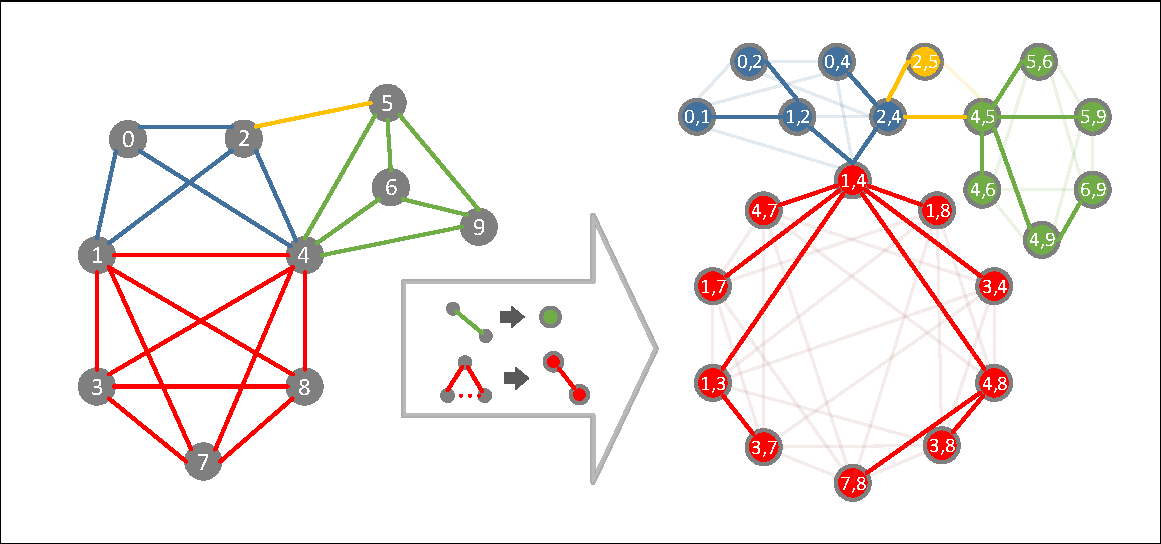
\includegraphics[width=0.8\linewidth, trim={0.1cm 0.1cm, 0.1cm, 0.1cm}, clip]{./figures/bottom_level.pdf}
    \caption{An example of the \inducedgraph{} and its maximum spanning tree of the example graph}
    \label{fig:\inducedgraph{}}
\end{figure}

We have the following theorem of vertex weights and edge weights in the \inducedgraph{}. 

\begin{Thm}
In \inducedgraph{} $G^m$, for a vertex $u$ and an adjacent edge $e$, we have $w_u \ge w_e$.
\label{thm:\inducedgraph{}_vertex_trussness}
\end{Thm}

\begin{proof}
According to \autoref{def:\inducedgraph{}}, $w_u$ is the trussness of the corresponding edge in $G_o$ while $w_e$ is the lowest trussness of edges in the corresponding triangle in $G_o$. 
%We have $\tau_{e} \ge \tau_{\triangle}$, therefore, $w_x \ge w_y$.
\end{proof}

We use $G^m$ to denote the maximum spanning forest of $G^t$ that has been stored as the bottom level index. To construct $G^m$, one way is generating the \inducedgraph{} $G^t$ first and then finding a maximum spanning tree of it. However, this approach is impractical because we need to sort edges in $G^t$ and the number of edges is three times the number of triangles of the original graph $G^o$, which can be an order of magnitude higher than the number of edges of most real-world graphs. We use two methods to avoid this. First, we find that for real-world graphs, the highest edge trussness is usually small compared to the size of the graph, \eg only a few thousand for the densest graph in our experiments. So we can use counting sort instead of comparison sort to reduce the time complexity. Second, as the weight of an edge of $G^t$ is the least trussness of edges in the corresponding triangle of $G^o$, we can sort edges of $G^o$ to generate edges of $G^t$ in sorted order with reduced space complexity. 
%This way, we can reduce the space complexity from $O(|{\triangle}^o|$ to $O({|E^o|})$. 
The details of the algorithm are shown in \autoref{alg:\inducedgraph{}_construction}. The algorithm takes $G^o$ and its edge trussness, which can be computed using the truss decomposition algorithm (\cite{wang2012truss}), as inputs.

\begin{algorithm}
	\KwData{$G^{o}(V^{o},E^{o})$, edge trussness $\{\tau_{e}, e \in E^{o}\}$}
	\KwResult{The \inducedgraph{} $G^{m}(V^{m}, E^{m})$}
	\BlankLine
	$sorted \gets$ sort edge trussness in decreasing order\;
	\For{$e \in E^{o}$} {
	   $V^{m} \gets V^{m} \bigcup \{e, \tau_{e}\}$\;
		 MAKE-SET($e$)\;
	}
	\For{$(u,v) \in sorted$}{
		suppose $u$ is the lower degree end of $(u,v)$\;
		\For{$w \in N_{u}$}{
			 \If{$(v,w) \in E^{o}$ \textbf{and} $\tau_{u,v} < \tau_{u,w}$ \textbf{and} $\tau_{u,v} < \tau_{v,w}$}{ 
				\Comment{Compare edge id if trussness of edges are equal to avoid duplication.}\;
				$\tau_{\triangle} = min(\tau_{(u,v)}, \tau_{(u,w)}, \tau_{(v,w)})$\;
				$E^{\triangle} \gets \{((u,v),(u,w)), \tau_{\triangle}\} \bigcup \{((u,v),(v,w)), \tau_{\triangle}\} \bigcup \{((u,w),(v,w)), \tau_{\triangle}\}$\;
				\For{$e^{\triangle} \in E^{\triangle}$}{
				  \If{FIND-SET($e^{\triangle}.v_1$) $\neq$ FIND-SET($e^{\triangle}.v_2$)}{
						$E^{m} \gets E^{m} \bigcup e^{\triangle}$\;
						UNION($e^{\triangle}.v_1$, $e^{\triangle}.v_2$)\;
					}
				}
			}
		}
	}
	\Return{$G^{m}(V^{m},E^{m})$}
	\caption{Bottom Level Index Construction}\label{alg:\inducedgraph{}_construction}
\end{algorithm}

The time and space complexity for computation of edge trussness of $G^o$ are $O(\sum_{(u,v) \in E^{o}}{min\{d_{u},d_{v}\}})$ and $O(|E^{o}|)$,  respectively. Sorting all the edges with counting sort costs $O(|E^{o}| + k_{max})$ time and $O(|E^{o}| + k_{max})$ space. The time and space complexity for listing all the triangles in $G^o$ is $O(\sum_{(u,v) \in E^{o}}{min\{d_{u},d_{v}\}})$ and $O(1)$, respectively. So the time and space complexity for generating the bottom level index when $k_{max} \ll |E^{o}|$ is $O(\sum_{(u,v) \in E^{o}} {min\{d_{u},d_{v}\}})$ and $O(|E^{o}|)$,  respectively. Since $G^m$ is a maximum spanning forest, the bottom level index takes $O(|V^{m}|) = O(|E^{o}|)$ space to store it.

\subsection{\TreeIndex{}}
\label{top-level}

\begin{figure}[ht]
    \centering
    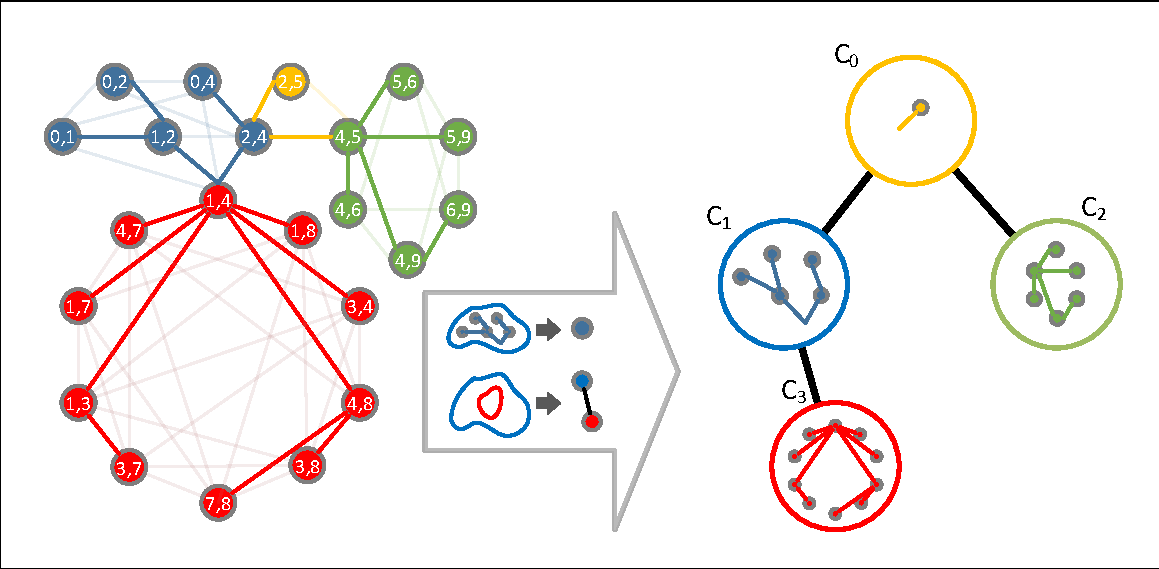
\includegraphics[width=0.8\linewidth, trim={0.1cm 0.1cm, 0.1cm, 0.1cm}, clip]{./figures/top_level.pdf}
    \caption{Overall structure of the \twolevelindex{}.}
    \label{fig:top-level}
\end{figure}

The top level index is extracted from k-truss communities and their relations in the original graph $G^o$ for fast locating relevant k-truss communities at query time. It is a super-graph having vertices represent unique k-truss communities and edges represent containment relations between k-truss communities. We call this index structure the \treeindex{} and denote it as $G^c$. Based on the hierarchical property of k-truss (\cite{cohen2008trusses}), \ie for $k \ge 2$, each $k$-truss is the subgraph of a ($k-1$)-truss, we have the formal definition of the \treeindex{} in \autoref{def:\treeindex{}}.

\begin{Def}[\Treeindex{}]
The \treeindex{} $G^c$ is a weighted undirected graph that each k-truss community in the original graph $G^o$ is represented by a vertex in $G^c$. $G^c$ has an edge $e^c$ connecting vertices $v^{c}_{1}, v^{c}_{2} \in G^{t}$ if and only if the following two conditions are met for their corresponding k-truss communities $C^{o}_{1}, C^{o}_{2} \in G^{o}$:
\begin{itemize}
	\item $C^{o}_{1}$ is a subgraph of $C^{o}_{2}$ or the other way around.
	\item Assume without loss of generality that $C^{o}_{1}$ is a subgraph of $C^{o}_{2}$, there is no $C^{o}_{3} \in G^{o}$ such that $C^{o}_{1}$ is a subgraph of $C^{o}_{3}$ and $C^{o}_{3}$ is a subgraph of $C^{o}_{2}$.
\end{itemize}
$G^c$ only has vertex weights, which are the trussness of the corresponding k-truss communities.
\label{def:\treeindex{}}
\end{Def}

A key property of the \treeindex{} is that it is a forest. 
%To prove this, we start with \autoref{thm:truss_hierarchy} 

%\begin{Thm}
%If k-truss community $C_{k1}$ is the subgraph of two other k-truss communities $C_{k2}$ and $C_{k3}$, respectively. We have $k2 \neq k3$.
%\label{thm:truss_hierarchy}
%\end{Thm}
%
%\begin{proof}
%According to \autoref{def:k-truss_community}, a k-truss community $C_{k1}$ is a subgraph of another k-truss community $C_{k2}$ when $C_{k1}$ and $C_{k2}$ are triangle connected and $k2 < k1$. Edges in $C_{k2}$ and $C_{k3}$ are triangle connected as they share the same k-truss community $C_{k1}$ as their subgraph. Suppose $k2 = k3$, $C_{k2} \bigcup C_{k3}$ meets the definition of k-truss community and becomes a larger k-truss community. This contradicts with $C_{k2}$ and $C_{k3}$ are maximal k-truss themselves.
%\end{proof}

\begin{Thm}
The \treeindex{} $G^c$ is a forest.
\label{thm:forest}
\end{Thm}

\begin{proof}
First, if there is a cycle $v^{c}_{1} ... v^{c}_{i} ... v^{c}_{n}$ in the \treeindex{} $G^c$ and their corresponding k-truss community in the original graph $G^o$ is $C^{o}_{1} ... C^{o}_{i} ... C^{o}_{n}$, respectively. According to \autoref{def:k-truss_community} and \autoref{def:\treeindex{}}, $C^{o}_{1} ... C^{o}_{i} ... C^{o}_{n}$ are triangle connected, and it is impossible for an arbitrary pair of community to have same trussness, as it contradicts with the maximal property of k-truss communities. Assume without loss of generality that vertex $v^{c}_{i}$ has the largest weight in this cycle, \ie its corresponding k-truss community $C^{o}_{i}$ has the smallest trussness. We denote the two adjacent vertices of it as $v^{c}_{j}$ and $v^{c}_{k}$. The corresponding k-truss communities are $C^{o}_{j}$ and $C^{o}_{k}$, respectively. By \autoref{def:\treeindex{}}, $C^{o}_{j}$ and $C^{o}_{k}$ are triangle connected. Assume without loss of generality that $C^{o}_{k}$ has smaller trussness than $C^{o}_{j}$, we have $C^{o}_{i}$ is a subgraph of $C^{o}_{j}$ and $C^{o}_{j}$ is a subgraph of $C^{o}_{k}$. So the edge between $v^{c}_{i}$ and $v^{c}_{k}$ contradict with the definition of the \treeindex{}.

Second, $G^c$ may have multiple connected components as not all k-truss communities in $G^o$ are triangle connected. 
\end{proof}

The \treeindex{} can be easily constructed with a single BFS traversal on the \inducedgraph{} $G^m$. For each connected component in $G^m$, the algorithm create a tree in the \treeindex{} $G^c$. The algorithm also creates a lookup table $H$ to map each vertex in $G^m$ to the super vertex in $G^c$ to which it belongs. \autoref{alg:\treeindex{}_construction} shows the detailed procedure. %Note that according to \autoref{thm:\inducedgraph{}_vertex_trussness}, an edge's weight is always smaller than it's endpoints' weights.

To construct each tree in $G^c$ with a connected component in $G^m$, the algorithm iteratively processes vertices during the BFS traversal and tracks the parent vertex $p^m$ of each vertex $u^m$.
To process a vertex $u^m$, the algorithm first compares weights, which are the trussness of corresponding edges in original graph $G^o$, of $u^m$ to its parent vertex $p^m$. The algorithm retrieves the super vertex $v^{c}_{p}$ using lookup table $H$, and find an ancestor super vertex with weight, which is trussness of the corresponding k-truss community in the original graph, smaller than the weight of $u^m$ if necessary. Depends on the relations of the weight of the found super vertex, the weight of the edge $(p^m, u^m)$ and the weight of vertex $u^m$, the algorithm decides whether to create a new super vertex in $G^c$ or assign $u^m$ to an existing super vertex.

\begin{algorithm}
	\KwData{$G^{m}(V^{m},E^{m})$}
	\KwResult{$G^{c}(V^{c},E^{c})$, $H$}
	\SetKwProg{Fn}{function}{}{end}
	\SetKw{Continue}{continue}
	\SetKw{Break}{break}
	\BlankLine
	%$Q \gets \emptyset$, $bfsparent \gets \emptyset$, $unvisited \gets V^{m}$\;
	%\While{$unvisited \neq \emptyset$}{
		%$seed \gets$ $unvisited.pop()$, $Q \gets Q \bigcup seed$; \Comment{Seed for new tree.}\
	\For{each connected component $CC \in G^m$} {
		$v^{m}_{seed} \gets CC.pop()$\;
		create\_super\_vertex($seed$, $null$)\;
		%\While{$Q \neq \emptyset$}{
			%$u^m = Q.pop()$\;
			%\For{$v^m \in N_{u^m} \bigcup unvisited$}{
				%$Q \gets Q \bigcup v^{m}$, $bfsparent[v^{m}] \gets u^{m}$, $unvisited.remove(v^{m})$\;
			%}
		\For{$u^m \in$ BFS starting at $seed$} {
			$p^m \gets$ parent of $u^m$ in BFS\;
			$e^m \gets (u^m, p^m)$\;
			$v^{c}_{p} \gets H[p^m]$\;
			%$p^m \gets bfsparent[u^m]$, $e^m \gets (u^m, p^m)$, $v^{s}_{p} \gets H[p^m]$\;
			\lWhile{$\tau_{v^{c}_{p}} > \tau_{e^m}$}{
				%\uIf{$\tau_{v^{s}_{p}} > \tau_{e^m}$}{
					${v^{c}_{p}}^{\prime} \gets v^{c}_{p}$, $v^{c}_{p} \gets v^{c}_{p}.parent$
					%\Continue
			}
			\eIf{$\tau_{v^{c}_{p}} < \tau_{e^m}$}{
				\eIf{$\tau_{e^m} = \tau_{u^m}$}{
					$v^{c}_{u} \gets$ create\_super\_vertex($u$, $v^{c}_{p}$)\;
					${v^{c}_{p}}^{\prime}.parent \gets v^{c}_{u}$\;
				} {
					$v^{c}_{e} \gets$ create\_super\_vertex($e$, $v^{c}_{p}$)\; 
					$v^{c}_{u} \gets$ create\_super\_vertex($u$, $v^{c}_{e}$)\;
					${v^{c}_{p}}^{\prime}.parent \gets v^{c}_{e}$\;
				}
			} {
				\eIf{$\tau_{e^m} = \tau_{u^m}$}{
					$H[u^m] \gets v^{c}_{p}$\;
				} {
					$v^{c}_{u} \gets$ create\_super\_vertex($u$, $v^{c}_{p}$)\;
				}
			}
		}
	}
	\Return{$G^{c}(V^{c},E^{c})$, $H$}
	\BlankLine
	\Fn{create\_super\_vertex ($u^m$, $v^{c}_{p}$)}{
		create $v^{c}_{u}$, $H[u^m] \gets v^{c}_{u}$\;
		$v^{c}_{u}.parent \gets v^{c}_{p}$\;
		$V^c \gets V^c \bigcup v^{c}_{u}$\;
		\Return{$C_u$}
	}
	\caption{Top Level Index Construction}
	\label{alg:\treeindex{}_construction}
\end{algorithm}

The reason we use the weight of the edge between a vertex and its parent vertex as the reference when adding a vertex of $G^m$ to $G^c$ can be explained by \autoref{thm:k_le_edge_weight}. 

\begin{Thm}
For a vertex $u^m$ and its neighbor vertex $v^m$ in the \inducedgraph{} $G^m$, if their representing edges in $G^o$ belong to the same k-truss community with the trussness of $k$, then $k \le \tau_{(u^m,v^m)}$. 
\label{thm:k_le_edge_weight}
\end{Thm}

\begin{proof}
Since $G^m$ is the maximum spanning forest, it has the cycle property, \ie for any cycle in the \inducedgraph{} $G^t$, if the weight of an edge in the cycle is smaller than the individual weights of all the other edges in the cycle, then this edge cannot belong to a maximum spanning forest. So there is no path in $G^t$ between $u^m$ and $v^m$ that has all edges with weight higher than $\tau_{(u^m,v^m)}$. Let $e^{o}_{u}$ and $e^{o}_{v}$ be their corresponding edges in original graph $G_o$, then $e^{o}_{u}$ is not triangle connected to $e^{o}_{v}$ in $G^o$ with edges that have trussness greater than $\tau_{(u^m,v^m)}$. Therefore, it is not possible for $e^{o}_{u}$ and $e^{o}_{v}$ to exist in the same k-truss community with trussness greater than $\tau_{(u^m,v^m)}$.
\end{proof}

For each vertex of $G^m$, searching the ancestor super vertex in $G^c$ of its parent vertex in $G^m$ takes $O(k_{max})$ time, where $k_{max}$ is the highest trussness of k-truss communities in $G^o$. Since the index construction process is a BFS on a maximum spanning tree with $O(|E^o|)$ vertices, the \treeindex{} construction algorithm takes $O(k_{max}|E^o|)$ time. As each vertex in $G^c$ represents a k-truss community in $G^o$, and $G^c$ is a forest. The algorithm takes $O(|E^o|)$ space and the index size is $O(|E^o|)$. %Although in practice, the size of $G^c$ is much smaller than $O(m)$.
%
%\begin{figure}[ht]
    %\centering
    %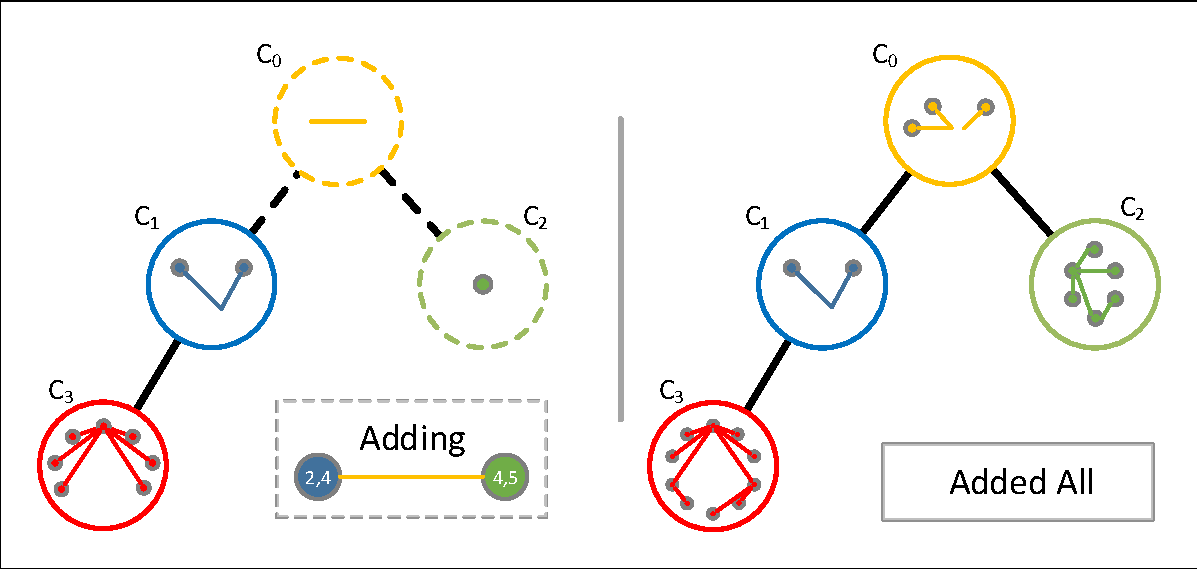
\includegraphics[width=\linewidth]{./figures/tree_index.pdf}
    %\caption{An example \treeindex{} of the \inducedgraph{} in \autoref{fig:\inducedgraph{}}}
    %\label{fig:\treeindex{}}
%\end{figure}
%
%An example is shown in \autoref{fig:\treeindex{}}

\subsection{\TwoLevelIndex Structure}
\label{structure}

\begin{figure}[ht]
    \centering
    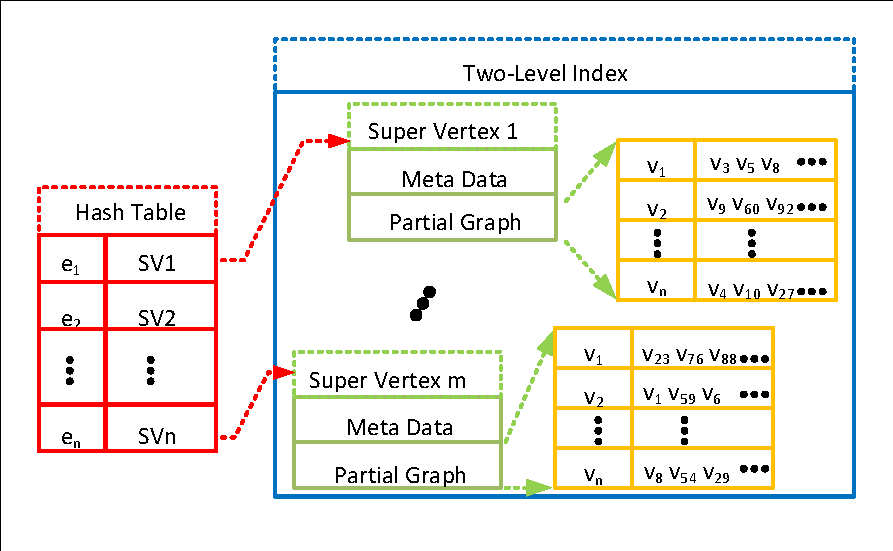
\includegraphics[width=0.8\linewidth, trim={0.1cm 0.1cm, 0.1cm, 0.1cm}, clip]{./figures/structure.pdf}
    \caption{Overall structure of the \twolevelindex{}.}
    \label{fig:structure}
\end{figure}

We combine the \inducedgraph{} and the \treeindex{} to form the \twolevelindex{} and arrange it in a structure that can provide information at different granularity. \autoref{fig:structure} shows an overview of the index structure. On the top level, we use an array to store the \treeindex{}. Each entry represents a single super vertex. Super edges are expressed by parent and children pointers. Within each entry, it also stores meta-data of the corresponding k-truss community, \eg the trussness, the community size, etc, for fast information retrieval. This meta-data can be gathered as a byproduct of index construction process. Finally, each entry contains a pointer of the data structure that stores part of the bottom level index. 

The bottom level index, which is the \inducedgraph{}, is stored as several separated adjacent lists. Each adjacent list contains edges of a single k-truss community that does not belong to any of its children k-truss communities. These adjacent lists can be easily generated as byproducts when constructing \treeindex{} using \autoref{alg:\treeindex{}_construction}. 
%Note that a vertex or edge in the \inducedgraph{} may belong to multiple k-truss communities. In these k-truss communities, k-truss communities with higher trussness is subgraphs of k-truss communities with lower trussness. To avoid redundancy, we only store the vertex and edge in the adjacent list of the k-truss community with the highest trussness. 

Finally, we have a hash table that maps each edge in the original graph to an entry in the top level of the \twolevelindex{}. One can also follow the similar fashion used in \cite{akbas2017truss}, which maps each vertex in the original graph to multiple entries in the top level index so that the original graph is not required during query time.
